%%%%%%%%%%%%%%%%%%%%%%%%%%%%%%%%%%%%%%%%%%%%%%%%%%%%%%%%
%%%%%%%%%------RMIT SPACE POSTER------------%%%%%%%%%%%%
%%%%%%%%%%%%%%%%%%%%%%%%%%%%%%%%%%%%%%%%%%%%%%%%%%%%%%%%
%%%%%%%%%%%%%%%%%%%%%%%%%%%%%%%%%%%%%%%%%%%%%%%%%%%%%%%%
% a0poster Portrait Poster
%
% The a0poster class was created by:
% Gerlinde Kettl and Matthias Weiser (tex@kettl.de)
% 
% License:
% CC BY-NC-SA 3.0 (http://creativecommons.org/licenses/by-nc-sa/3.0/)
%
% Author/Designer: Timothy Kodikara
%
%% Note: CRC and SERC logos are included in the /figures folder if you might want to use them.
%%%%%%%%%%%%%%%%%%%%%%%%%%%%%%%%%%%%%%%%%
%----------------------------------------------------------------------------------------
%	PACKAGES AND OTHER DOCUMENT CONFIGURATIONS
%----------------------------------------------------------------------------------------
\documentclass[a0,portrait]{a0poster}
%%
\title{Sketches Pos}
\usepackage[top=5cm, bottom=0.3cm, left=5cm, right=3cm]{geometry}
\usepackage[compact]{titlesec}
\usepackage{multicol} % This is so we can have multiple columns of text side-by-side
\columnsep=100pt % This is the amount of white space between the columns in the poster
\columnseprule=15pt % This is the thickness of the blue line between the columns in the poster
\usepackage{subfig}
\usepackage{float}
\usepackage[svgnames]{xcolor} % Specify colors by their 'svgnames', for a full list of all colors available see here: http://www.latextemplates.com/svgnames-colors
%\usepackage{times} % Use the times font
\usepackage{palatino} % Uncomment to use the Palatino font
\usepackage{xkeyval}
\usepackage{graphicx} % Required for including images
\setlength{\abovecaptionskip}{5pt plus 5pt minus 3pt}
\graphicspath{{figures/}} % Location of the graphics files
\usepackage{booktabs} % Top and bottom rules for table
\usepackage[font=small,labelfont=bf]{caption} % Required for specifying captions to tables and figures
\usepackage{amsfonts, amsmath, amsthm, amssymb} % For math fonts, symbols and environments
\usepackage{csquotes}
\usepackage{wrapfig} % Allows wrapping text around tables and figures
%\usepackage[pdftex]{color}
\usepackage{algorithm}
\usepackage{algcompatible}
\usepackage[noend]{algpseudocode}
\def\columnseprulecolor{\color{NavyBlue}}%
\usepackage{framed}
\colorlet{frameborder}{NavyBlue}

\newcommand\Fontvi{\fontsize{21}{10}\selectfont}

%----------------------------------------------------------------------------------------
%	POSTER HEADER 
%----------------------------------------------------------------------------------------
% The header is divided into three boxes:
% The widths of these boxes can be easily edited to accommodate your content as you see fit
\begin{document}
%\hspace*{0.2cm}
\begin{minipage}[c]{\linewidth}
\vspace{0.1cm}
\noindent\makebox[\textwidth][c]{
\begin{minipage}[c]{0.10\linewidth}
\vspace{0pt}\raggedright
\hspace{1cm}

\includegraphics[width=2\linewidth]{pure-logo}
\end{minipage}
\hfill
\begin{minipage}[c]{0.70\textwidth}
\centering
\Huge \color{NavyBlue} \textbf{Vectorized Hashing for Sketches}\\[0.5cm]
\large \color{Black} \textbf{Fatih Tasyaran, Kerem Yildirir,Hakan Ogan Alpar,Ali Osman Berk Supervised by  Kamer Kaya}\\[0.2cm] % Author(s)
\small Sabanci University, Faculty of Engineering and Natural Sciences\\[0.1cm] % University
\small Computer Science and Engineering\\[0.1cm] % Affiliation 2
\end{minipage}
%\hfill
\begin{minipage}[c]{0.15\textwidth}
\vspace{0pt}\raggedleft

\includegraphics[scale=2,width=\linewidth]{suLogo.jpg}
\hspace{1cm}
\end{minipage}}
\\[0.1cm]%
% A bit of extra whitespace between the header and poster content
%----------------------------------------------------------------------------------------
\color{NavyBlue}\setlength\FrameRule{25pt}
\begin{framed}
\Fontvi
\vspace{0.5cm}
\begin{multicols}{2} % This is how many columns your poster will be broken into, a portrait poster is generally split into 2 columns
%----------------------------------------------------------------------------------------
%	INTRODUCTION
%----------------------------------------------------------------------------------------
\color{Black}
\section*{Introduction}
Searching is one of the most important problems of computer science and it is used extensively in many areas. Hash functions are one-way functions that map an input value to another value. Randomness is essential in hashing because it is not desired to have multiple values resulting in the same hash value. Hashing is also used in  data structures where we use the hashed values as indexes of a table  and keep the value in the index of a table determined by hash function. This property allows us to do search, insert, delete operations in O(1) time. \cite{NIPS2017_7239}
%----------------------------------------------------------------------------------------
%	METHODS
%---------------------------------------------------------------------------------------- 
\color{Black}
\section{Intel SIMD Instructions}
SIMD is an instruction set available mostly on all current processors. In this project we used AVX (Advanced Vector Extension) and AVX2 instructions which are available for Intel processors since Sandy Bridge architecture. With AVX instructions, it is possible to process 128 bits of data in registers on parallel, with AVX2 this increased to 256 bits, meaning that we can do simple arithmetic and logical operations of 8 32-bit integers at the same time.\cite{Wang:2014:SPF:2568058.2568059}

\color{Black}

% begin{figure}[H]
% \centering

% \subfloat[Tabular Hash implemented in C++]{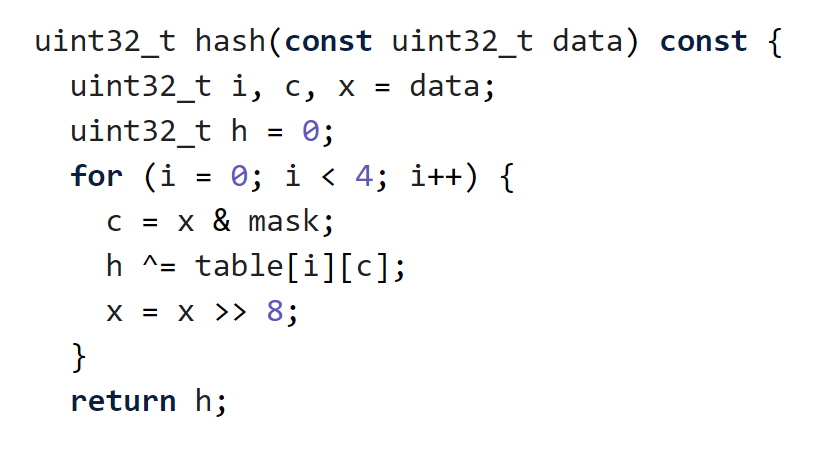
\includegraphics[width=0.5\linewidth]{figures/tabular_code.png}}
% \subfloat[Count min sketch illustration]{\includegraphics[width=0.55\linewidth]{figures/countmin.png}}


% \end{figure}\
% \section*{Tabular Hash}
% In data sketches, elements that inserted to the table must be hashed multiple times. In our implementations of sketching, we used tabular hashing. It is a strong hash function
% which grants significant level of randomness. Hashing process requires a table filled with random integers. After initializing the table, hash function can be used.
% With using the fastest known hashing scheme multiplication-shift hashing. Hash function takes an 32-bit integer  as input. It divides  into 4
% 8-bit chunks and iterates them in order. At each iteration, logical AND operation is done between the element and an 8-bit mask which consists of zeros. With this, it is guaranteed that first 8-bits of the 32-bit integer becomes zero. This also changes the value of element $x$ to another integer . Then, logical XOR operation is applied between changed element and the integer in hash table which is on the $ith$ row where $ 0\leq i \leq 4 $ and $cth$    column and assigned to a variable $h$.\par


% %\vspace{0.1cm}
% \begin{center}
% 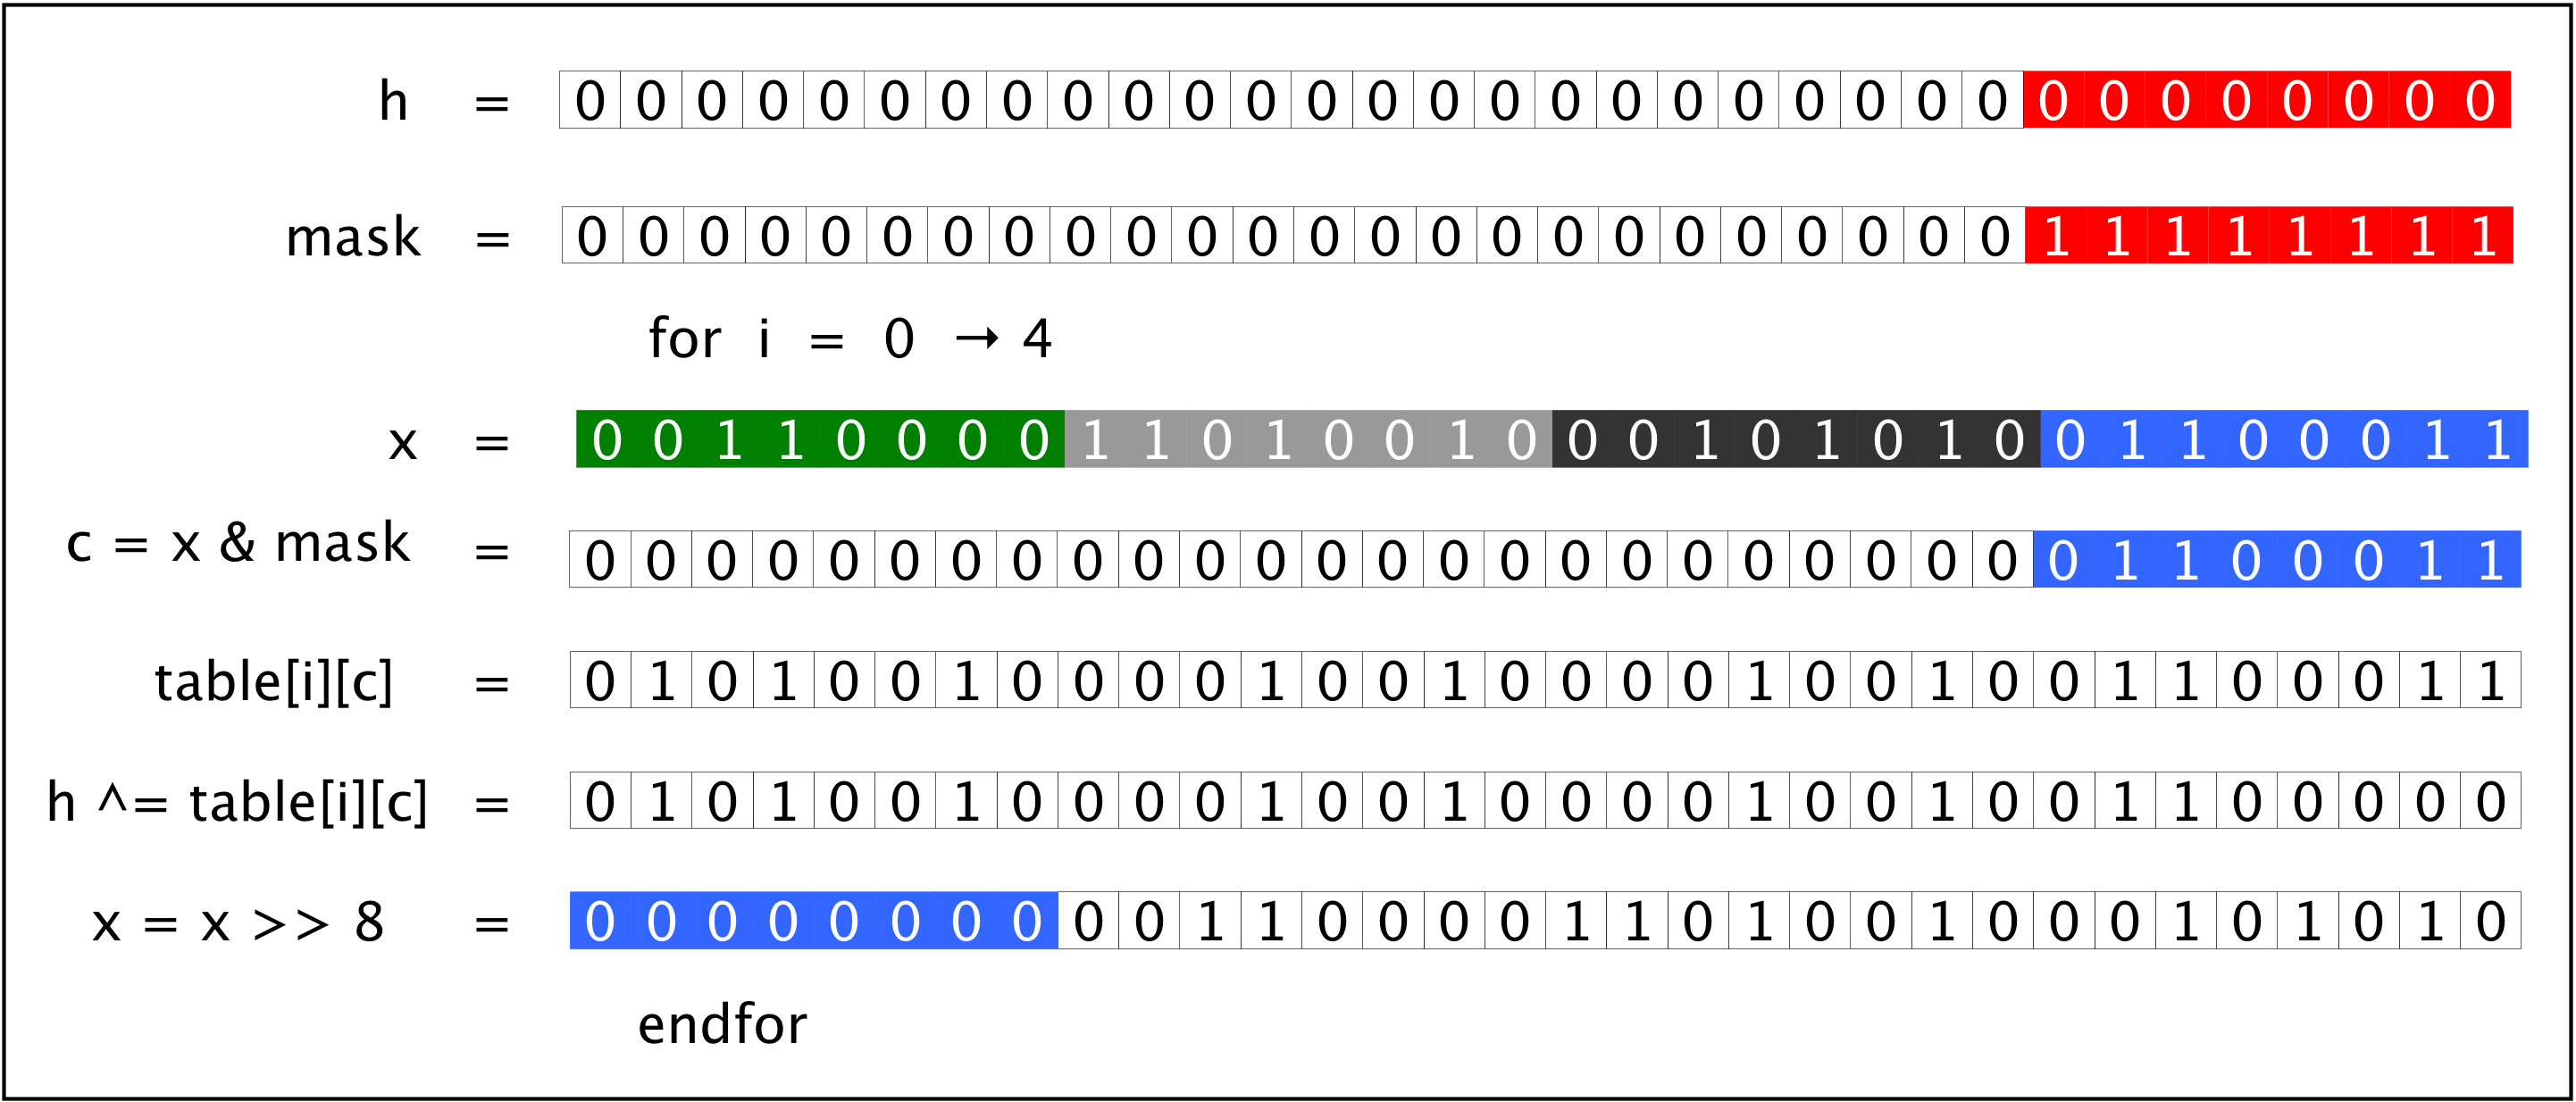
\includegraphics[width=\linewidth]{figures/tabularHash}
% \captionof{figure}{\color{Green}Tabular Hash illustrated}
% \label{GIMlatlon}
% \end{center}
% At the end of iteration,  is shifted right 8-bits. When all iterations are done a unique $h$ value has been achieved. 

%----------------------------------------------------------------------------------------
%	CONCLUSIONS
%----------------------------------------------------------------------------------------
\color{Black}
\section{Hashing Strategies}
As our hash functions, we used Multiply-Shift Hash, MurMurHash3  and Tabular Hash. Pseudocodes of these functions can be found in Appendix B. For each hash function, we have developed our work under 2 models; Model 1, one data multiple hash, where we generate multiple hash values from a single data sample, and Model 2, one data one hash, where we generate only one hash value using the same random seed for a single data sample. For both models we implemented the hash functions with SIMD instructions in simple arithmetic and logical operations. This way we were able to process 8 32-bit integers in parallel.
\subsection{Model 1}
\begin{figure}[H]
\centering
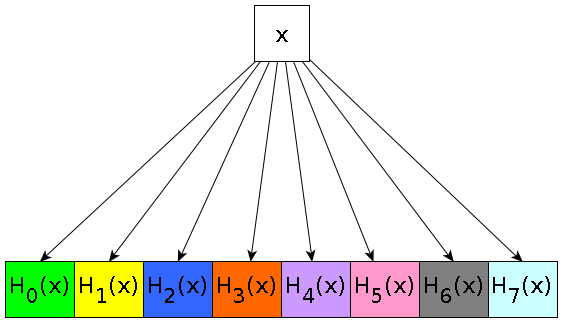
\includegraphics[width=0.24\textwidth]{one_data_multi_hash.png} 
\caption{Illustration of Model 1}
\end{figure}
First model computes 8 hash values for a single given input. We apply the hash function using 8 different random seeds and do all the operations using these random 8 values. We fill an array of size 8 with our input value and apply the operation with 8 different random seeds. This model is especially useful for algorithms like Count-Min Sketch where we keep multiple hash values for a single element. 
\subsection{Model 2}
\begin{figure}[H]
\centering
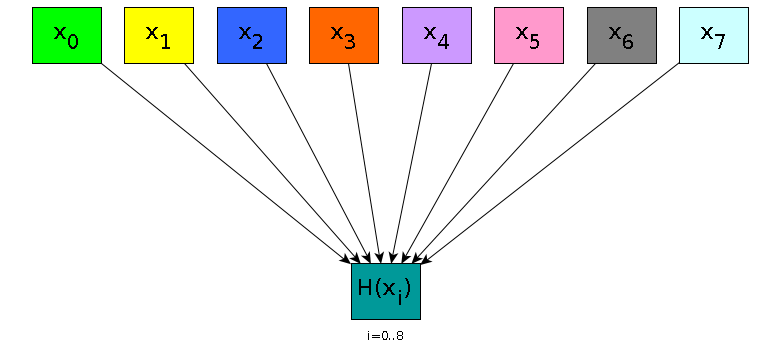
\includegraphics[width=0.3\textwidth]{multi_data_single_hash.png} 
\caption{Illustration of Model 2}
\end{figure}
Second model computes 8 hash values for given 8 inputs, using the same random seed for all data points. This approach could be seen as overriding the data length a register can hold, which is 256 bits, by carrying 8 different 32-bit value to get 8 different 32-bit hash result by single instruction, in parallel. Using this approach, the goal is to achieve 8 hash values in a time of 1 hash value without SIMD instructions. This approach could be useful in applications like bloom filter, where every element needs one hash to check membership to a set.


\section{Tabular Hash SIMD}
Tabulation hashing is a simple but relatively powerful hash function due to its randomness and efficiency \cite{DBLP:journals/corr/abs-1011-5200}. The algorithm is the
following;
Let p be the key to be hashed, m be the desired bit length of hash output. M is a k * n
matrix and used as a lookup table. Matrix has m bit random elements in every cell.
%
% \begin{algorithm}
% \begin{algorithmic}

% \end{algorithmic}
% \end{algorithm}
%
This algorithm returns a single hash value corresponding to a given single p
(key). It is possible to construct two models which are able to return multiple hash
values $f_i(p)(i=0,1,…)$ corresponding to a given a single p and return a multiple
hash values as a result of same hash function $f_0 (p i ) (i=0,1,2,3….)$ corresponding
to given different p’s (as a vector) by using SIMD instructions and vectors.
The first model takes a single p value as key, but uses a lookup table which has a
different type. The algorithm returns a vector of m bit hash values. Initialization of
M is the difference between this algorithm and the original one. M contains
vectors of random m bits as elements. The speedup is a result of parallel XOR
operations.

The other model uses same type of lookup table M But XOR and shifting
operations are done by using SIMD ınstructions. Algorithm takes a vector of p
values as different keys. The result is again a vector of different m bit hash
values.
%%
%%
\begin{algorithm}[H]
\begin{algorithmic}
\Function{Simple Tabulation Hash}{p,m,M}
\State Given p,m, and initialized M(k*n)
\State hashvalue=0
\For{ every i th most significant q bit of p, call it x}
\State hashvalue = hashvalue  $\oplus$ M[i][x]
\EndFor
\Return hashvalue

\EndFunction


\Function{Tabular Hash SIMD}{p,m,M(k * n)}
\State Given p, m, M(k * n)
\State  hashvalue= [0,0,…..0]
\For{ every ith most significant q bit of p, call it x}
\State hashvalue = \_mm256\_xor\_si256(hashvalue, M[i][x]) 
\EndFor
\Return hashvalue
\EndFunction

\end{algorithmic}
\end{algorithm}
% %%
%%
\section{Experiment and Results}
\begin{figure}[H]
    \centering
    \subfloat[Tabular Hash with $2^{30}$ elements]{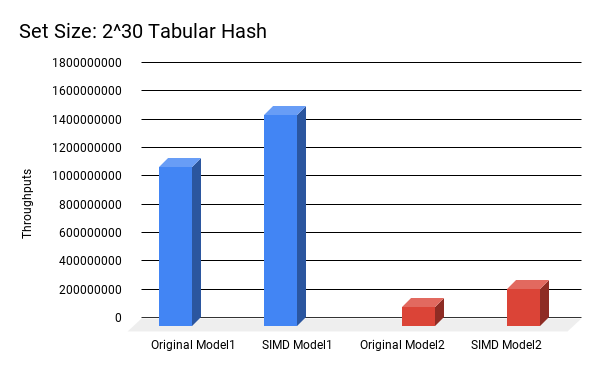
\includegraphics[width=0.4\linewidth]{tb30.png}}   
     \hspace{1em}
    \subfloat[Tabular Hash with $2^{25}$ elements]{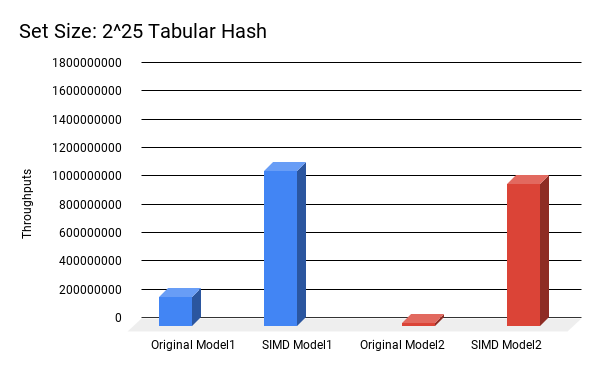
\includegraphics[width=0.4\linewidth]{25tb.png}}
    \label{fig:my_label}
\end{figure}
\begin{figure}[H]
    \centering
    \subfloat[Multiply Shift Hash with $2^{25}$ elements]{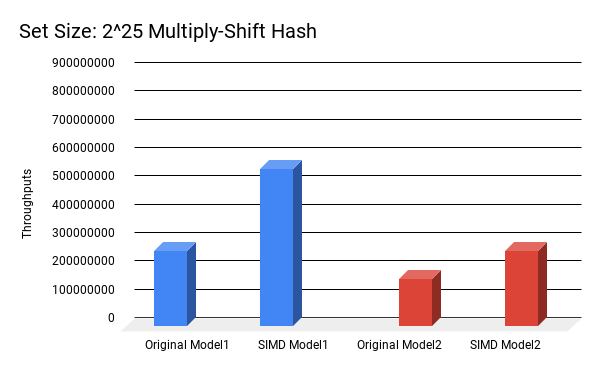
\includegraphics[width=0.4\linewidth]{25ms.png}}
     \hspace{1em}
    \subfloat[Multiply Shift Hash with $2^{30}$ elements]{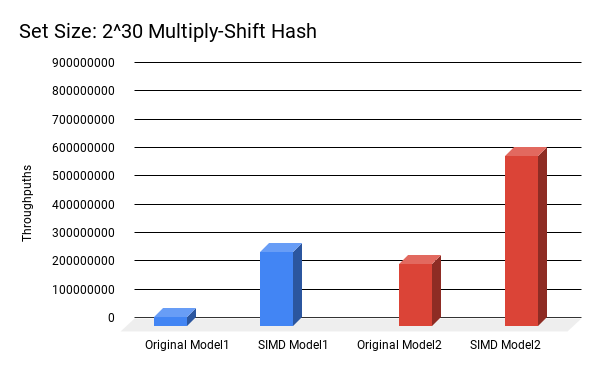
\includegraphics[width=0.4\linewidth]{ms30.png}}
\end{figure}
\begin{figure}[H]
    \centering
    \subfloat[Murmur Hash with $2^{30}$ elements]{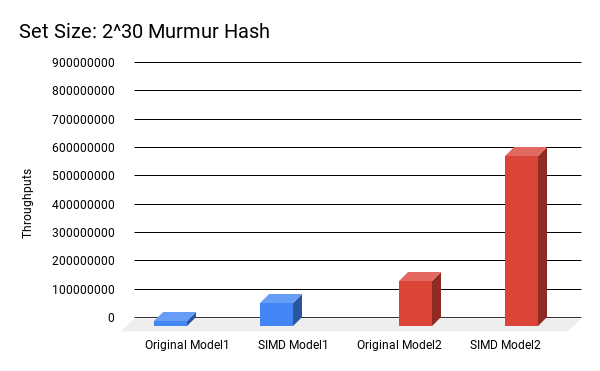
\includegraphics[width=0.4\linewidth]{mumrur30.png}}
        \hspace{1em}
  \subfloat[Murmur Hash with $2^{25}$ elements]{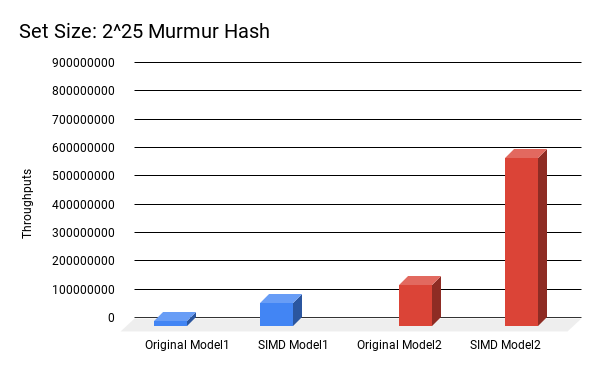
\includegraphics[width=0.4\linewidth]{mumru25.png}}

    
    \label{fig:my_label}
\end{figure}
Above figures demonstrate the throughputs achieved using SIMD instructions in each hashing function. Main speed is due to shift and xor operations with SIMD instructions. There is a bottleneck on load and extract operations which slows down the process.
\section{Future Work}
In the future, we plan to use our hash functions with SIMD instructions in probabilistic data structures and algorithms such as HyperLogLog, Bloom Filter and Count-Min Sketch. These algorithms are very useful in estimating frequencies in large data streams.  We believe that parallelizing the hashing operations in these algorithms  will provide great amount of speedup in frequency estimation. 
\subsection{HyperLogLog}
HyperLogLog hashes every key to a bit stream and then approximates the distinct element number of the hashed set by bit stream's prefixes. To do this, HyperLogLog uses the same hash function for all keys to be hashed. With this property, HyperLogLog is suitable for multiple data, one hash approach. 
Implementing SIMD instructions on a HyperLogLog could achieve great speedup as the HyperLogLog works in a one pass over data manner, only counting hash values.
\subsection{Bloom Filter}
As mentioned earlier, bloom filter is one of the well suited applications for multiple data - one hash approach. To open up, bloom filter is a membership query which hashes keys to hash values and map them in a bit vector. With a bloom filter employing a SIMD instruction including hash function, it would be possible to answer 8 membership queries at once.
\begin{figure}[H]
\centering
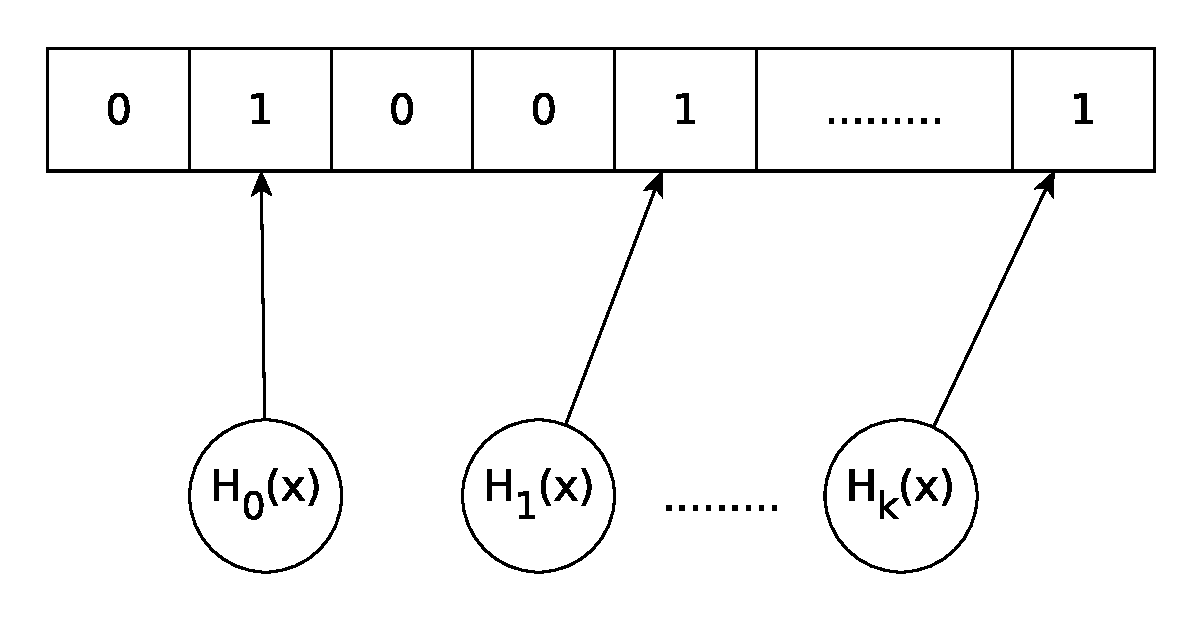
\includegraphics[width=0.24\textwidth]{bloom.eps}
\caption{Illustration of an insertion of the element $x$ to a bloom filter with k hash functions}
\end{figure}
\subsection{Count-Min Sketch}
Count-min sketch is a perfectly well suited application to use with one data multiple hash approach. Since a count-min sketch is basically a 2 dimensional matrix, the rows of which are 1 dimensional hash tables. To insert an element to a sketch (i.e. counting it) requires different hash values for each row of the count-min sketch. By using  SIMD instructions, calculating hash values for all rows a sketch at a time could achieve a promising speed-up for the hashing phase of a count-min sketch.
\begin{figure}[H]
\centering
\includegraphics[width=0.24\textwidth]{countmin.png}
\caption{Illustration of Count-Min Sketch}
\end{figure}
% \begin{center}


% \fbox{ 
% \begin{minipage}{30em}
% \textbf{SoC}: Broadcom BCM2837\par
% \textbf{CPU}: 4× ARM Cortex-A53, 1.2GHz\par
% \textbf{GPU}: Broadcom VideoCore IV\par
% \vspace{1mm}
% \textbf{RAM}: 1GB LPDDR2 (900 MHz)\par
% \textbf{Networking}: 10/100 Ethernet, 2.4GHz 802.11n wireless\par
% \textbf{Bluetooth}: Bluetooth 4.1 Classic, Bluetooth Low Energy\par
% \textbf{Storage}: 16 GB Class10 microSD\par
% \textbf{GPIO}: 40-pin header, populated\par
% \textbf{Ports}: HDMI, 3.5mm analogue audio-video jack, 4× USB 2.0, Ethernet, Camera Serial Interface (CSI), Display Serial Interface (DSI)
% \end{minipage}
% }
% \end{center}


\bibliographystyle{ieeetr}
\bibliography{mybib.bib}
\end{multicols}
%\textcolor{NavyBlue}{\rule{\linewidth}{15pt}}
\vspace{0.5cm}
\end{framed}
\end{minipage}
%\hspace*{0.1cm}
\end{document}
%----------------------------------------------------------------------------------------
%%%%%%%%%%%%%%%%%%%%%%%%%%%%%%%%%%%%%%%%%%%%%%%%%%